\documentclass{beamer}
%\pgfpagesuselayout{2 on 1}[a4paper,portrait,border shrink=5mm]
%\pgfpagesuselayout{8 on 1}[a4paper,portrait,border shrink=5mm]

\usepackage{../fhnw-beamer}

\date{\today}
\author{rolf.schmutz@fhnw.ch}
\institute{FHNW}
\title {Netzwerke und Datenkommunikation}

\usepackage{verbatim}
\usepackage{amsmath}
\usepackage{yfonts}

\begin{document} % ===============================================================

\begin{frame}
\begin{tiny}
\begin{itemize}
  \item picture example of L2-network not scaling
  \item picture intermediate device L2 interprets L2-addresses but does not change it
  \item L2 addresses are device-addresses (just a bunch of devices), L3 are ``logical'' (synthetic) addresses giving a meaning of localisation/group
  \item L3 allows every device to determine if a destination is {\em local} or {\em remote} (and only reachable via gateway)
  \item picture of L3 device interpreting L3 but not changing it
  \item picture of a whole lot of intermediate L3/router with seperate L2 in-between
\end{itemize}
\end{tiny}
\end{frame}

\begin{frame}
\frametitle{L2 revisited (1/2)}
\includegraphics[width=11cm]{L2-base-network.pdf}
\end{frame}

\begin{frame}
\frametitle{L2 revisited (2/2)}
\includegraphics[width=10cm]{L2-base-network-L2-gateway.pdf}
\end{frame}

\begin{frame}
\frametitle{L2 Intermediate Device Operation (Bridge)}
\includegraphics[width=10cm]{L2_intermediate-device}
\end{frame}

\begin{frame}
\frametitle{L3 Intermediate Device Operation (Router)}
\includegraphics[width=10cm]{L3_intermediate-device}
\end{frame}

\section{ND04: IP Layer-3}
\subsection{\"Ubersicht}

\begin{frame}
\frametitle{L3 Objectives}
\begin{itemize}
	\item{Sie kennen die Unterschiede Layer-2 zu Layer-3 Adressierung}
	\item{Sie kennen die Strukturierung der Layer-3 Adressen in (Sub-) Netze}
	\item{Sie wissen, dass IP/Layer-3 ein {\em paketvermittelndes} Netz darstellt}
	\item{Sie verstehen das Konzept der {\em Netzmasken} und k\"onnen es anwenden}
	\item{Sie wissen wie Layer-3 Pakete {\em geroutet}\footnote{Wegleitung im Internet}werden}
	\item{Sie wissen, dass IP/Layer-3 nach dem {\em best-effort} Prinzip arbeitet und die Zustellung der Pakete nicht garantiert ist}
\end{itemize}
\end{frame}


\begin{frame}
\frametitle{L3 Stack}
\includegraphics[width=12cm]{stack-overview-3}

Header:
\begin{itemize}
  \item{\emph{global} g\"ultige \emph{End-zu-End} (Ger\"ate) Adressierung}
  \item{\emph{Header}-Pr\"ufsumme\footnote{d.h. keine Pr\"ufsumme \"uber die SDU}}
  \item{Flags, Fragment, ``Lebensdauer'', Unters\"utzung f\"ur (einfache) Qualit\"atsicherung etc}
  \item{\ldots und nat\"urlich das ``upper-level-protocol''}
\end{itemize}
\end{frame}


\begin{frame}
\frametitle{L3 Factlets}
\begin{itemize}
	\item{Layer-3 verbindet Systeme {\em End-to-End} \footnote{im Gegensatz zu Layer-2, das nur Teilstrecken/benachbarte Systeme verbindet} -- d.h. weltweit}
	\item{Layer-3 Adressen sind {\em strukturiert} in (Sub-) Netze\footnote{wie z.B. das Telefon-Netzwerk}}
	\item{IP/Layer-3 ist ein {\em paketvermittelndes} Netz: die Nutzdaten werden paketisiert und gesondert \"ubertragen}
	\item{verschiedene Layer-3 Netzwerke werden durch {\em Router}\footnote{oder ``Gateway'' (ungenauer)} miteinander verbunden}
	\item{die Dateneinheit auf IP/Layer-3 ist das Paket ``packet''\footnote{bei Layer-2 war das ``frame''}}
	\item{die Zustellung der Pakete auf IP/Layer-3 ist nicht garantiert\footnote{im Gegensatz zu Ethernet/L2 kann aber L3 bereits Fehlermeldungen zum Kommunikationspartner ausl\"osen -- \emph{wenn} die Header-Checksum stimmt\ldots}}
\end{itemize}
\end{frame}

\begin{frame}
\frametitle{Unterschiede Layer-2 zu Layer-3 Adressierung}
\begin{itemize}
	\item{Layer-2 ist eine {\em Ger\"ate-Identifikation}\footnote{wie z.B. die AHV-Nummer} {\em ohne} Struktur/Lokationsinformation}
	\item{ein Internet\footnote{weltweiter Netzwerkverbund} w\"are mit Layer-2 Adressen nicht m\"oglich, da die Bridge-Tabellen zu gross w\"urden}
	\item{Layer-3/IP fasst mehrere Ger\"ate in einem IP-(Sub-) Netz zusammen\footnote{wie bei den Telefonnummern die Landesvorwahl/Ortsvorwahl} und erlaubt so eine effiziente lokalisierung}
	\item{\"uber Layer-3/IP ist so eine weltweite lokalisierung/addressierung von {\em Endger\"aten} m\"oglich}
\end{itemize}
\end{frame}

\begin{frame}
\frametitle{Paketvermittelndes Netz}
\begin{itemize}
	\item{Layer-3 unterteilt die Nutzdaten\footnote{z.B. Webseiten oder Bild- und Tondaten} in kleinere Einheiten und versendet diese gesondert \"uber das Netz\footnote{wie auch schon auf Layer-2}}
	\item{Die Pakete k\"onnen verloren gehen oder in anderer Reihenfolge\footnote{oder auch {\em verdoppelt} werden} am Ziel ankommen -- die Wiederherstellung der Nutzdaten ist Aufgabe der oberen Layer}
	\item{ein paketvermittelndes Netz ist Fehlerresistent\footnote{solange die oberen Layer f\"ur die garantierte Zustellung aufkommen. Der Ausfall einzelner Verbindungen/L2 im Internet ist \"ublicherweise kein Problem}}
	\item{\ldots und erlaubt eine effiziente Auslastung\footnote{im Gegensatz zu leitungsvermittelnden Netzen -- wo die Reservierung der Bandbreite unabh\"angig der tats\"achlichen Ausnutzung erfolgt} der Resourcen}
\end{itemize}
\end{frame}


\begin{frame}
\frametitle{Struktur der IP-Adressen ``(Sub-) Netzwerke''\footnote{im Folgenden werden ``Subnetze'' und ``Netze'' weitgehend Synonym verwendet}}
\begin{itemize}
	\item{IP-Adressen bestehen aus 32-Bit und werden \"ublicherweise im ``dotted-decimal''\footnote{4-Bytes im Dezimalformat 0-255 getrennt durch ``.''} Format notiert: {\texttt 194.41.161.1}}
\end{itemize}
  {\center 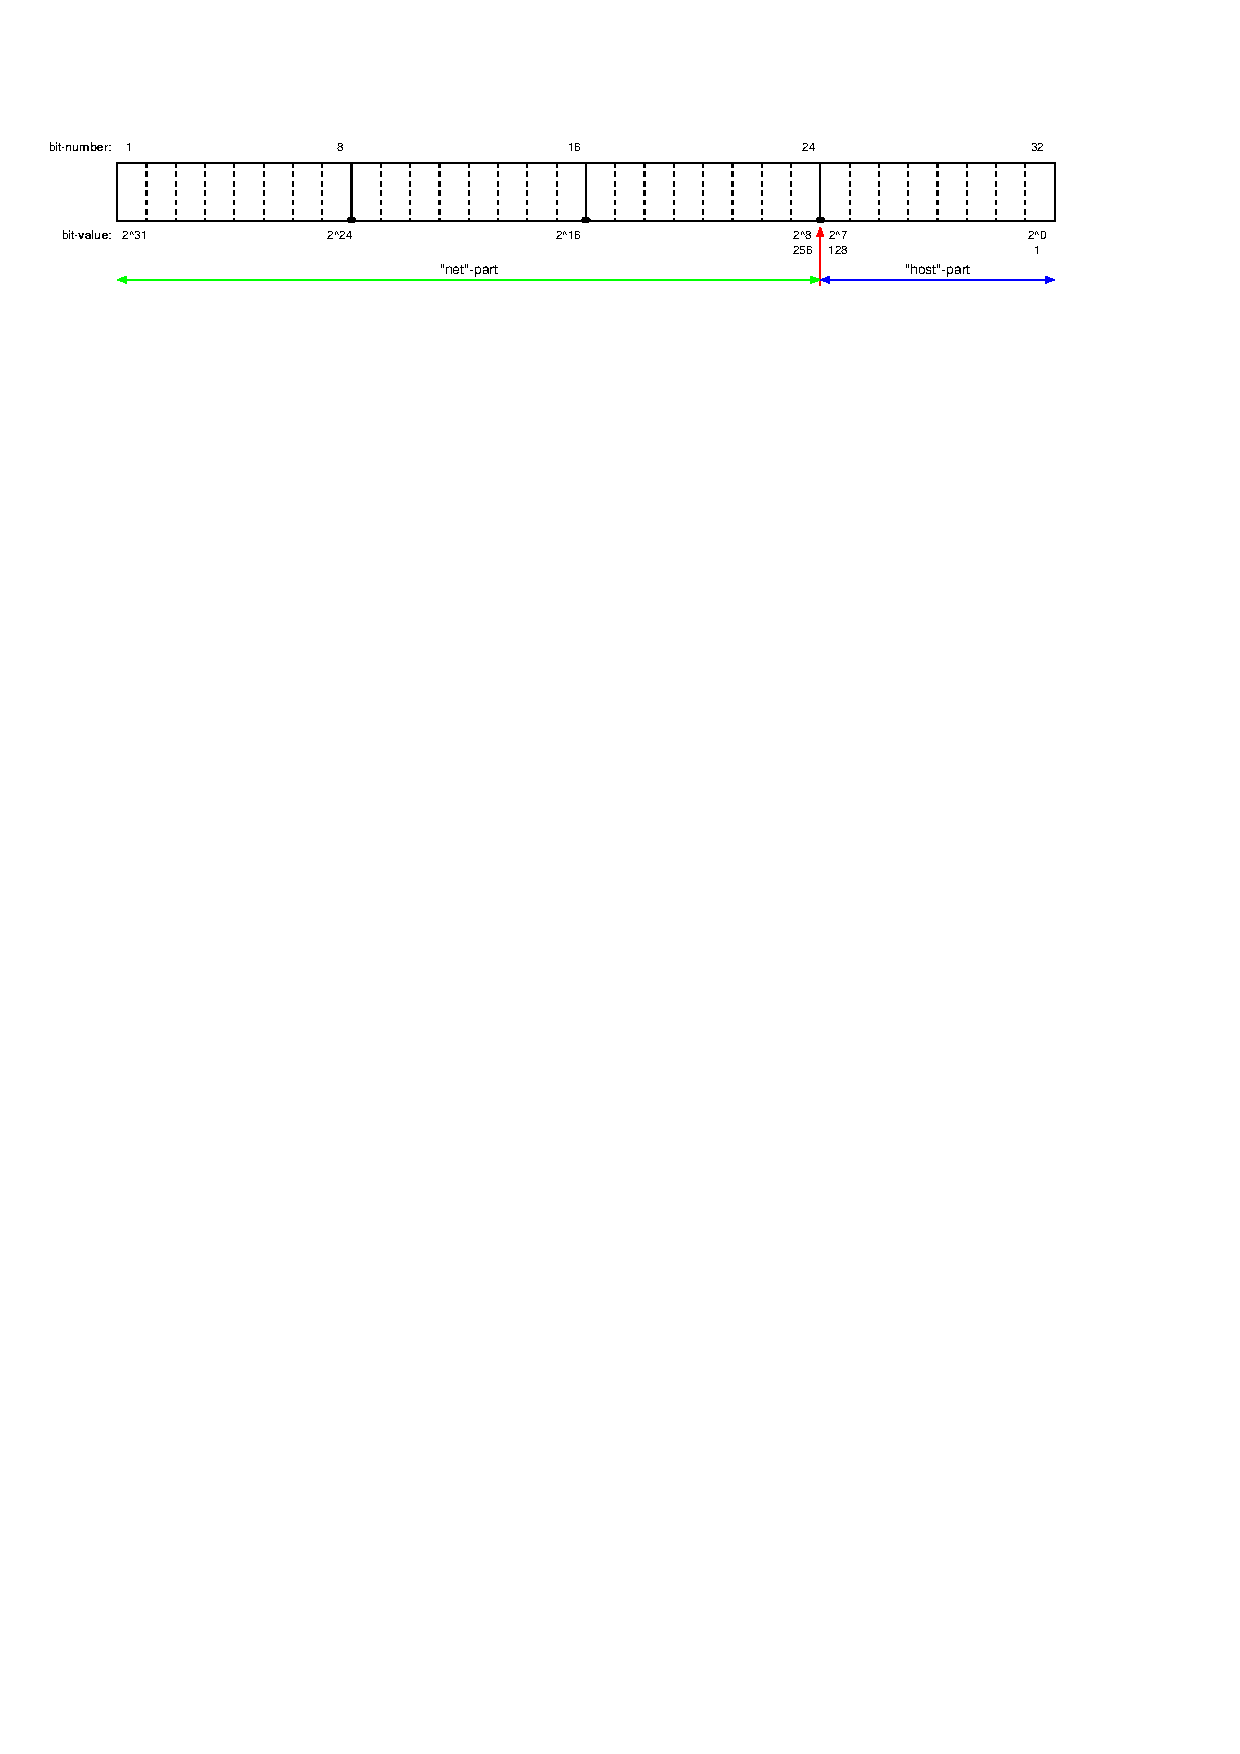
\includegraphics[height=1.6cm]{ip-address}}
\begin{itemize}
	\item{die 32-Bit werden in {\em Netz-} und {\em Host-}Anteil unterteilt\footnote{manchmal zus\"atzlich in Sub-Netz-Anteil}}
	\begin{itemize}
	\item{{\tiny Netz: entspricht etwa Landes-, Ortsvorwahl im Telefonnetz}}
	\item{{\tiny Host: entspricht etwa Nummer des Telefonapparates ohne Vorwahl}}
  \end{itemize}
  \item{Das ``routing''\footnote{Wegleitung} wird aufgrund des Netz-Anteils bestimmt}
  \begin{itemize}
	\item{{\tiny \ldots wie beim Telenfonnetz\ldots}}
\end{itemize}
	\end{itemize}
\end{frame}

\begin{frame}
\frametitle{Netz-Anteil}
\begin{itemize}
	\item{der Netz-Anteil kann mittels {\em Netzmasken} oder {\em Pr\"afixl\"angen} angegeben werden:}
	\begin{itemize}
	\item{{\tiny bit-and Maske im ``dotted-decimal'' Format: {\textbf {\texttt 255.255.255.0}}, bin\"ar: {\textbf {\texttt 11111111.11111111.11111111.00000000}}}}
	\item{{\tiny Pr\"afixl\"ange (Anzahl gesetzter=``1'' Bits\footnote{``consecutive 1-bits from MSB''} in der Maske): {\textbf {\texttt /24}}}}
\end{itemize}
\item{Netzzugeh\"origkeit: wird mittels der logischen ``Bitwise-And'' Operation durchgef\"uhrt}
\begin{itemize}
	\item{{\tiny IP-Adresse in bin\"ares Format umrechnen, eg: {\texttt 192.168.1.5}$_{10}$$\rightarrow${\texttt 11000000.10101000.00000001.00000101}$_{2}$}}
	\item{{\tiny IP-Maske in bin\"ares Format verwandeln, eg: {\texttt 255.255.255.0}$_{10}$$\rightarrow${\texttt 11111111.11111111.11111111.00000000}$_{2}$}}
	\item{{\tiny ``bitwise-and'' Verkn\"upfung von IP-Adresse und -Maske, eg:\\{\texttt 11000000.10101000.00000001.00000101}$_{2}$ {\textbf \&} {\texttt 11111111.11111111.11111111.00000000}$_{2}$ $=$\\{\texttt 11000000.10101000.00000001.00000{\textbf 0}0{\textbf 0}}$_{2}$ $\rightarrow$ {\texttt 192.168.1.{\textbf 0}}$_{10}$
	}} 
	\item{{\tiny \ldots die so gewonnene Adresse wird als {\em Netzbasisadresse} bezeichnet und kann {\em nicht} f\"ur ein Endger\"at/Node verwendet werden}}
\end{itemize}
\item{der Host-Anteil kann auf gleiche Weise gewonnen werden, wenn die Maske zuerst {\em invertiert}\footnote{``one's-complement''} wird}
\end{itemize}
\end{frame}


\begin{frame}
\frametitle{Interlude}
\begin{itemize}
	\item{finden Sie die IP-Adresse und die Netzmaske Ihres Laptops\footnote{{\texttt ifconfig}/{\texttt ipconfig}, {\texttt netstat -r}}}
	\item{bestimmen Sie aus diesen Informationen die {\em Netzbasisadresse} und den Host-Anteil}
	\item{bestimmen Sie ob die beiden IP-Adressen \texttt{192.168.2.126} und \texttt{192.168.2.130} bei Verwendung einer Netzmaske (f\"ur beide) von \texttt{255.255.255.128} im selben Netz liegen}
	\item{bestimmen Sie die Anzahl m\"oglicher\footnote{Gesamtanzahl minus zwei: broadcast und base} IP-Adressen bei Verwendung der Netzmasken \texttt{255.255.255.0} und \texttt{255.255.254.0}}
	\item{berechnen Sie die ``l\"angste''\footnote{d.h. das eben gerade ausrechende kleinste Netzwerk} Netzmaske wenn rund 2000 Adressen im selben Netz ben\"otigt werden}
\end{itemize}
\end{frame}


\begin{frame}
\frametitle{Aufteilung des Adressbereichs}
\begin{itemize}
  \item{bis ca 1993 ``chaotisch'': \myurl{http://www.iana.org/assignments/ipv4-address-space/ipv4-address-space.xml}}
  \item{seither (CIDR) in geographisch/institutionell hierarchischer Weise \"uber ``Unterverteiler'' RIR\footnote{regional-internet-registry, z.B. \myurl{http://www.ripe.net/}}, private Provider\footnote{z.B. 212.x.x.x und 213.x.x.x sind beide ``Europa'' -- \"ahnlich wie ``Landesvorwahl''}}
\end{itemize}
\end{frame}


\begin{frame}
\frametitle{IP-Adressbereich als Klassen ``{\Huge {\frakfamily ye olde way}}'' 1/2}
\begin{center}
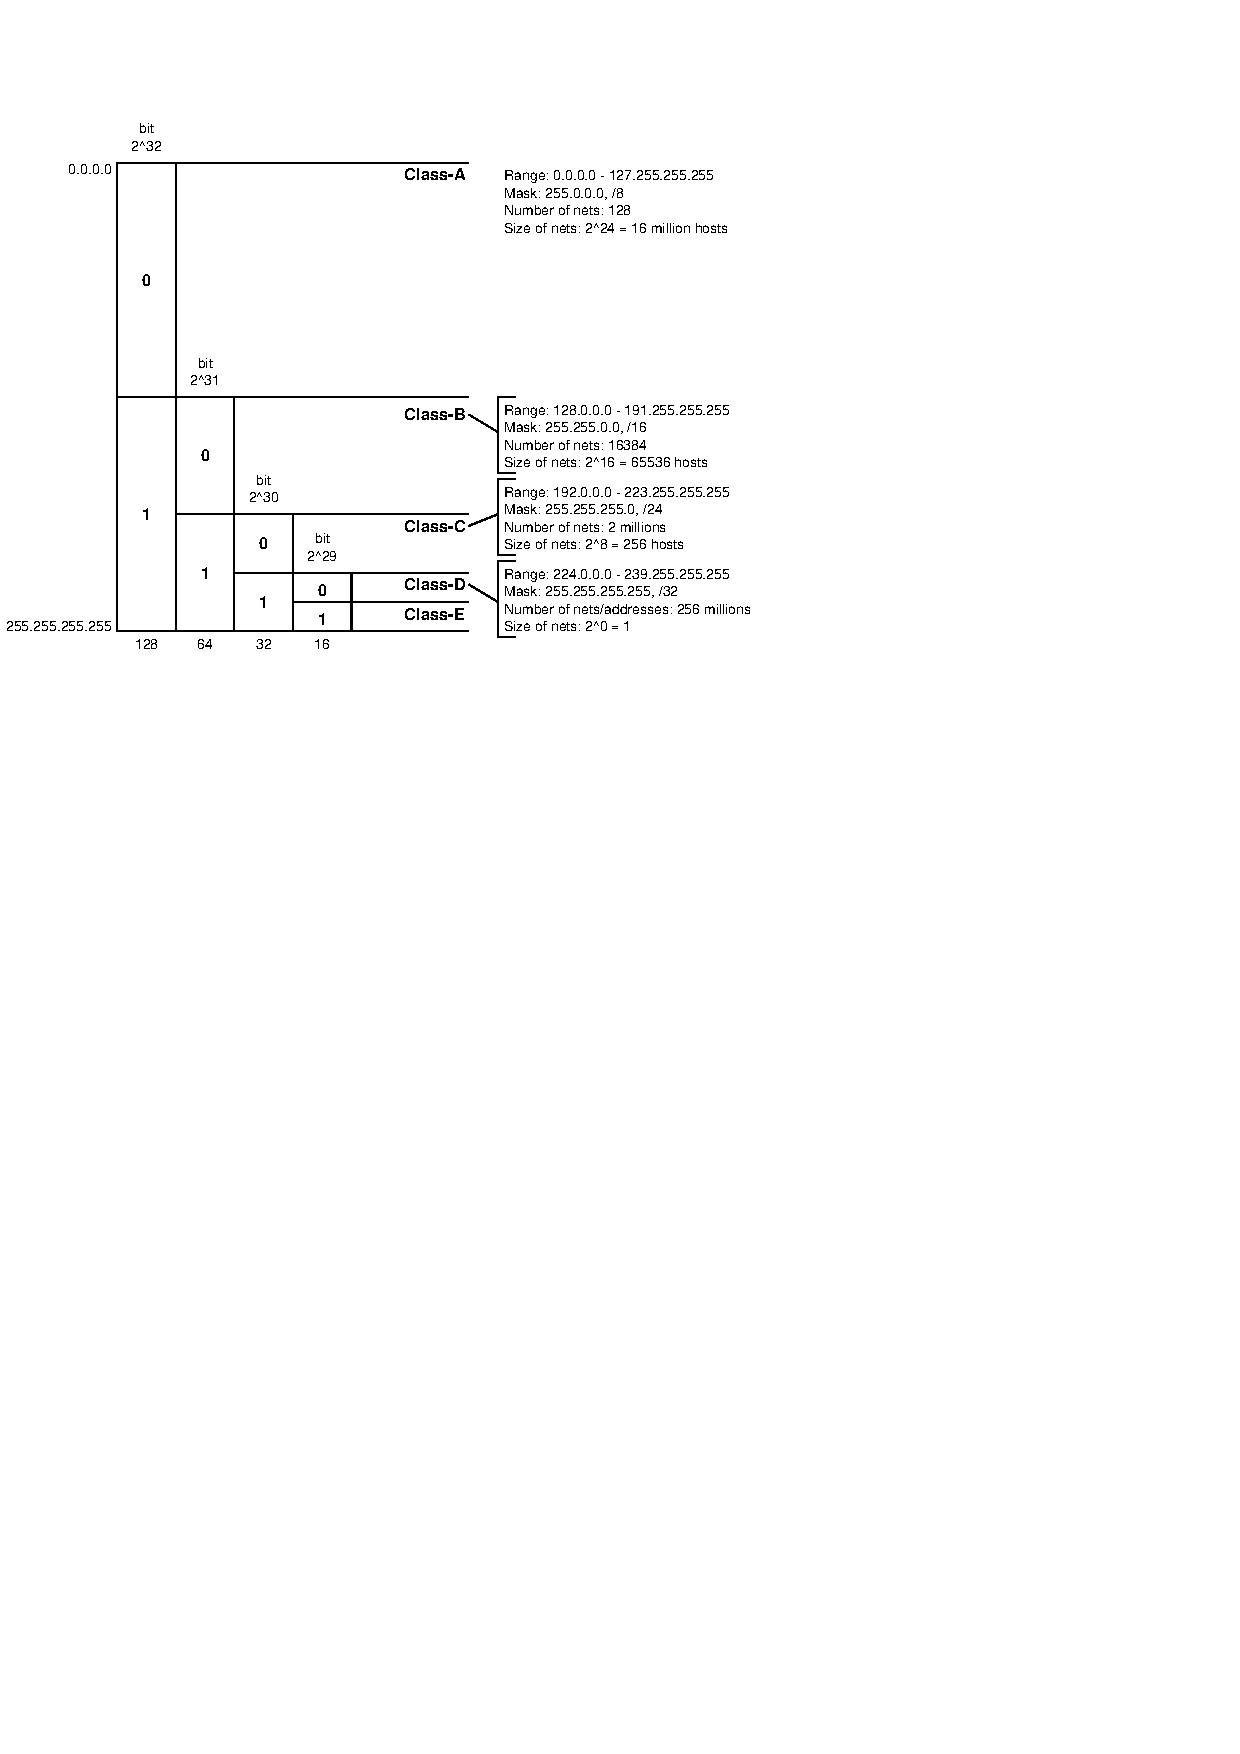
\includegraphics[height=21cm]{class-based}
\end{center}
\end{frame}

\begin{frame}
\frametitle{IP-Adressbereich als Klassen ``{\Huge {\frakfamily ye olde way}}'' 2/2}
\begin{itemize}
	\item{es werden mit {\em ID-Bits} identifizierte Adressbereiche f\"ur grosse, mittlere und kleine Netze gebildet}
	\item{\ldots ``it seemed a good idea in the 80\'{}''}
	\item{Problem-1: nur 128 Netze belegen die H\"alfte des Addressraums (aber k\"onnen 16 Millionen Hosts aufnehmen)}
	\item{Problem-2: keine topographisch/hierarchische\footnote{wie z.B. das Telefonnetz} Aufteilung}
	\item{Problem-3\footnote{big, fat\ldots}: Router m\"ussen im schlechtesten Fall etwas \"uber {\em 2 Millionen} Netze kennen}
\end{itemize}
\end{frame}

\begin{frame}
\frametitle{CIDR ``Classless Inter-Domain Routing'' (the new way) 1/2}
\begin{itemize}
	\item{Neustrukturierung\footnote{soweit m\"oglich\ldots Bereits zugewiesene Netze k\"onnen nicht entfernt werden} des Adressbereichs}
	\item{Klassen werden {\em nicht} mehr beachtet}
	\item{Bildung von {\em Supernetzen} f\"ur effizientes hierarchies routing\footnote{eg. {\texttt 212/7$\rightarrow$Europa}}\\$\rightarrow$ kleine Routing-Tables}
	\item{Bessere Ausnutzung des Adressbereichs durch Aufteilung der A- und B-Klassen in kleinere Einheiten}
  \item{Notation als {\em Pr\"afixl\"ange}\footnote{``slash''-Notation}: {\texttt 255.255.240.0}$\rightarrow${\texttt /20}}
\end{itemize}
\end{frame}

\begin{frame}
\frametitle{CIDR ``Classless Inter-Domain Routing'' (the new way) 2/2}
\begin{center}
\includegraphics[height=5.5cm]{bgp-growth.pdf}
\end{center}
{\tiny \verbatiminput{bgp-table-growth.sh}}
\end{frame}


\begin{frame}
\frametitle{\ldots noch mehr Spass mit Bits}
\begin{itemize}
\item{Berechnen Sie zu der CIDR-Pr\"afixl\"ange \texttt{/20} die entsprechende Netzmaske}
\item{\ldots und umgekehrt zu der Netzmaske \texttt{255.255.192.0} die Pr\"afixl\"ange}
\item{wieviele m\"ogliche IP-Adressen k\"onnen in \texttt{/21} untergebracht werden?}
\item{Bestimmen Sie ob die beiden IP-Adressen \texttt{172.17.71.5/23} und \texttt{172.17.70.240} im selben Netz liegen}
\end{itemize}
\end{frame}

\begin{frame}
\frametitle{Routing und Routing-Table}
\begin{itemize}
	\item{die Wegleitung ``routing'' im Internet:}
	\begin{itemize}
	\item{{\tiny wird bei jedem Router\footnote{``hop-by-hop'' und ``next-hop''} neu entschieden und dann an den n\"achsten Router oder an den Zielhost zugestellt}}
	\item{{\tiny entschieden wird der ``next-hop'' \"uber die {\em Routing-Tabelle}\footnote{im Folgdenen ``routing-table'' oder RT -- eigentlich ist das die FIB}}}
\end{itemize}
\item{die {\em Routing-Tabelle} enth\"alt (mindestens):}
\begin{itemize}
	\item{{\tiny {\em Ziel-Netz} (dest-net)}}
	\item{{\tiny {\em Ziel-Maske} oder {\em Ziel-Pr\"afixl\"ange} (dest-mask, prefixlength)}}
	\item{{\tiny {\em N\"achster-Router} (next-hop oder gateway)}}
\end{itemize}
\item{der {\em Routing-Vorgang} (forwarding): findet den ``next-hop'' f\"ur eine gegeben/empfangene IP-{\em Ziel}-Adresse (target-ip)}
\begin{itemize}
	\item{RT-Eintrag ``passt'', wenn: \\{\texttt ( target-ip {\textbf \&} dest-mask$_{i}$ ) = dest-net$_{i}$}, dann wird das Paket an {\texttt next-hop$_{i}$} weitergeleitet}
	\item{die RT wird nach Pr\"afixl\"ange in {\em absteigender} Reihenfolge konsultiert}
	\item{die ``Default-Route'' ist \texttt{0.0.0.0/0}}
\end{itemize}
\end{itemize}
\end{frame}



\begin{frame}
\frametitle{References}
\begin{itemize}
	\item{\myurl{http://en.wikipedia.org/wiki/IPv4_subnetting_reference}}
	\item{\myurl{http://en.wikipedia.org/wiki/Classless_Inter-Domain_Routing}}
	\item{Route-servers: \myurl{http://www.traceroute.org/\#Route\%20Servers}}
	\item{BGP-routing-table growth: \myurl{http://bgp.potaroo.net/as2.0/bgp-active.html}, andere lustige Informationen: \myurl{http://bgp.potaroo.net/as2.0/}}
	\item{CIDR: \myurl{http://books.google.ch/books?id=axiW1d8GosIC\&lpg=PA125\&pg=PA101\#v=onepage\&q=\&f=false}}
	\item{IP-address landscape: \myurl{http://xkcd.com/195/}}
\end{itemize}
\end{frame}



\end{document} 
